\documentclass[11pt]{beamer}  %% versione proiettore
%%\documentclass[11pt,handout]{beamer} %% versione stampa
\usepackage{lucidiJb-2ed}

\usepackage{relsize}

\mode<article>
{
  \usepackage{fullpage}
  \usepackage{hyperref}
}

\mode<presentation>
{
  \setbeamertemplate{background canvas}[vertical shading][bottom=red!10,top=blue!10]
  \usetheme{Ethereum}
  \usefonttheme[onlysmall]{structurebold}
}

\subtitle{Learning Ethereum}
\title{The Basics}
\institute{Universit\`a di Verona, Italy}
\date{January 2020}

\setbeamercovered{invisible}

\def\codesize{\smaller}
\def\<#1>{\codeid{#1}}
\newcommand{\codeid}[1]{\ifmmode{\mbox{\codesize\ttfamily{#1}}}\else{\codesize\ttfamily #1}\fi}

\begin{document}

\begin{frame}
  \titlepage
\end{frame}

\begin{frame}
  \frametitle{What is Ethereum?}

  \begin{greenbox}{}
    An open source, globally decentralized computing infrastructure
    that executes programs called \emph{smart contracts}, written
    in a Turing-complete programming language, translated into
    bytecode and run on a virtual machine. It uses a
    blockchain to synchronize and store the system's state changes
    (key/value tuples), along
    with a cryptocurrency called \emph{ether} to meter and constrain
    execution resource costs. It enables developers to build
    decentralized applications with built-in economic functions.
  \end{greenbox}

  \begin{itemize}
  \item \emph{gas} is bought when a transaction starts, with a threshold
    gas price
  \item DApps are smart contracts + web frontend (web3)
  \end{itemize}
  
\end{frame}

\begin{frame}\frametitle{People behind Ethereum}

  \begin{center}
  \begin{tabular}{c@{\hskip 1.5cm}c}
    
\includegraphics[scale=.3,clip=false]{pictures/vitalik_buterin.jpg} &
    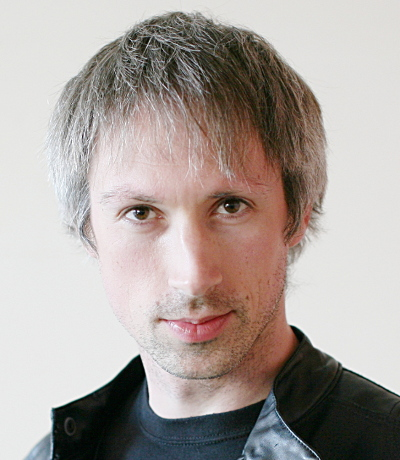
\includegraphics[scale=.247,clip=false]{pictures/gavin_wood.jpg} \\
    Vitalik Buterin & Gavin Wood
  \end{tabular}
  \end{center}
  
\end{frame}

\begin{frame}\frametitle{References used in this course}

  \begin{center}
  \begin{tabular}{c@{\hskip 1.5cm}c}
    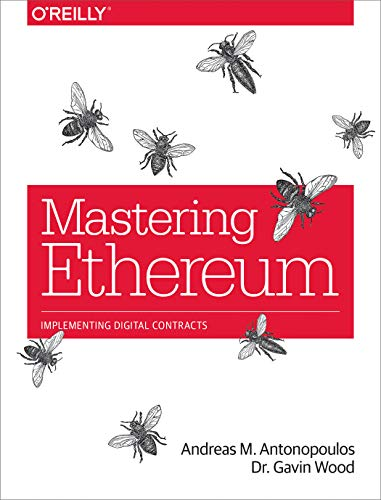
\includegraphics[scale=.3,clip=false]{pictures/mastering-ethereum.jpg} &
    
\includegraphics[scale=.3,clip=false]{pictures/building-games.jpg}
  \end{tabular}
  \end{center}

  The first: \url{https://github.com/ethereumbook/ethereumbook}

\end{frame}

\begin{frame}\frametitle{Ether (ETH) price over the years}

  \begin{center}
    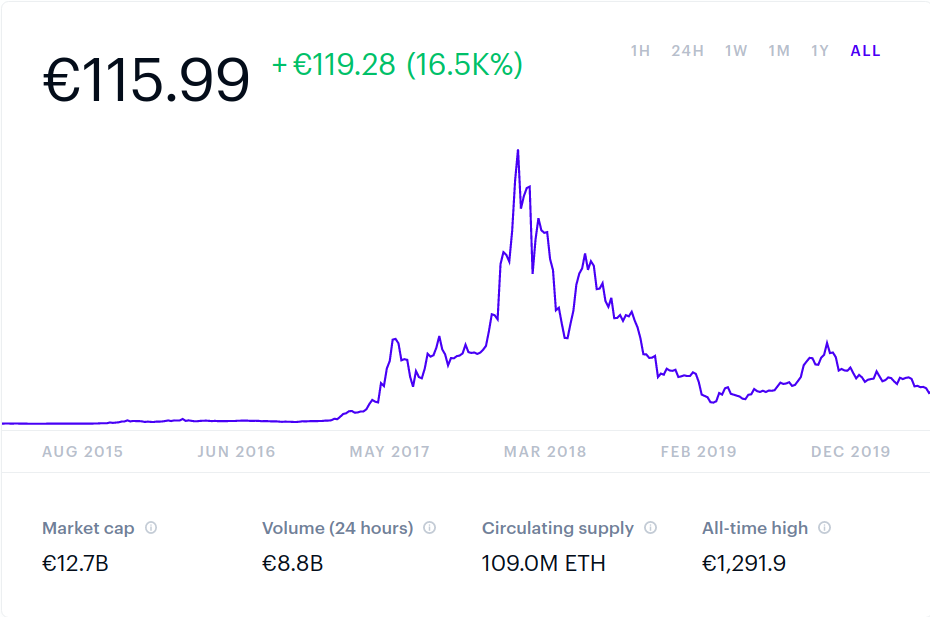
\includegraphics[scale=0.29,clip=false]{pictures/ethereum.png}
  \end{center}

\end{frame}

\begin{frame}\frametitle{Ethereum Classic Ether (ETC) price over the years}

  \begin{center}
    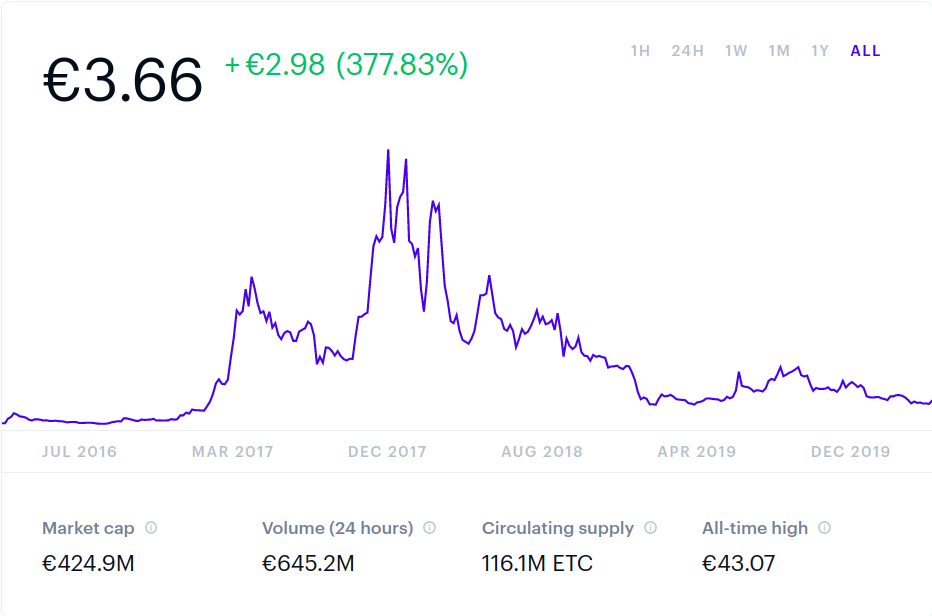
\includegraphics[scale=0.29,clip=false]{pictures/ethereum-classic.png}
  \end{center}

\end{frame}

\begin{frame}\frametitle{Ether denominations and unit names}

  \begin{center}
    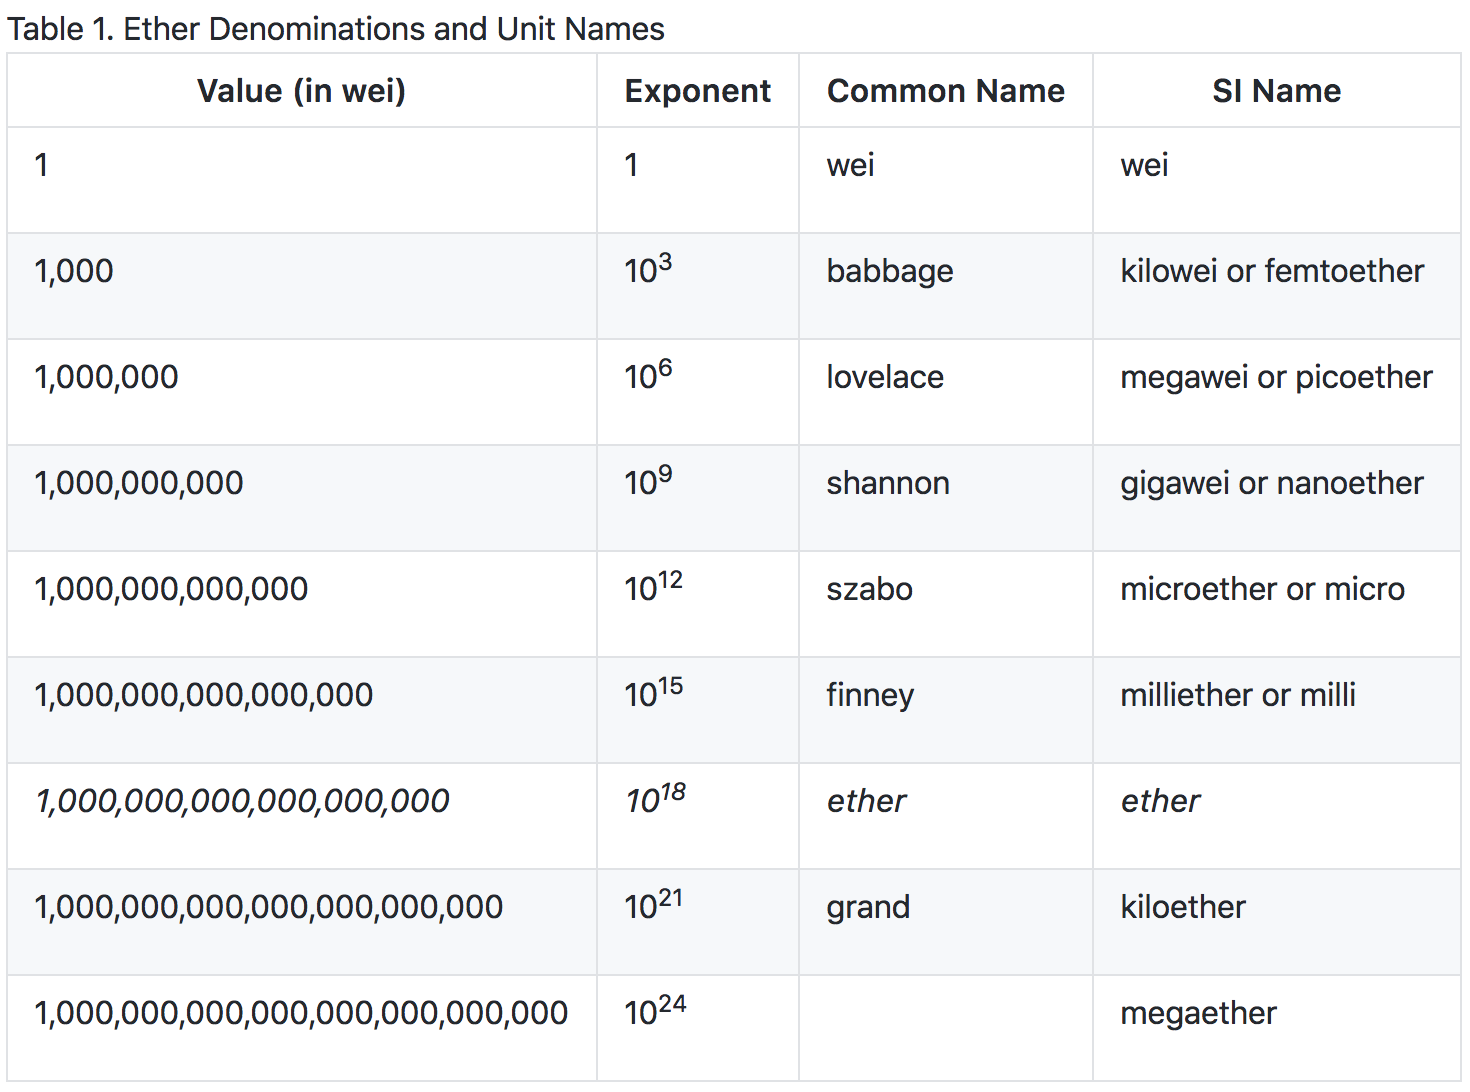
\includegraphics[scale=0.2,clip=false]{pictures/ether-denominations.png}
  \end{center}

\end{frame}

\begin{frame}\frametitle{Wallets}

  \begin{greenbox}{}
    A wallet is a
    software application that helps you manage your Ethereum account(s),
    by keeping your keys, creating and broadcasting transactions:
    \begin{itemize}
    \item mobile (Jaxx)
    \item desktop (Jaxx, Emerald Wallet)
    \item web-based (MetaMask, MyEtherWallet)
    \end{itemize}
  \end{greenbox}

\end{frame}

\begin{frame}\frametitle{MetaMask: create account}

  \begin{center}
    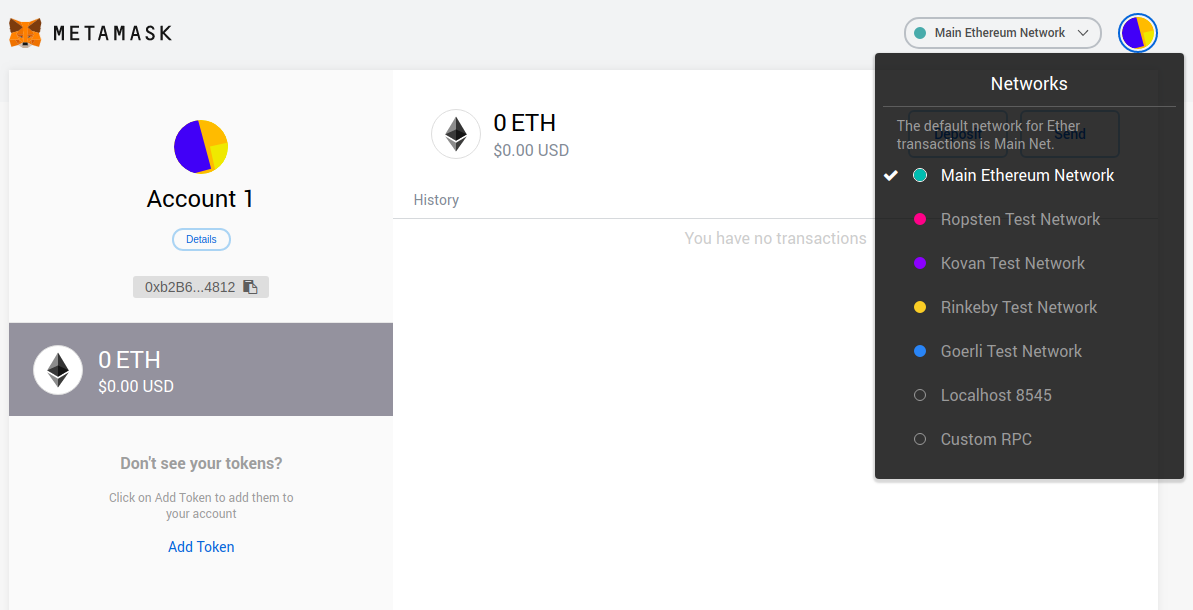
\includegraphics[width=\textwidth,clip=false]{pictures/metamask-account.png}
  \end{center}

\end{frame}

\begin{frame}\frametitle{MetaMask: connect to the faucet}

  \begin{center}
    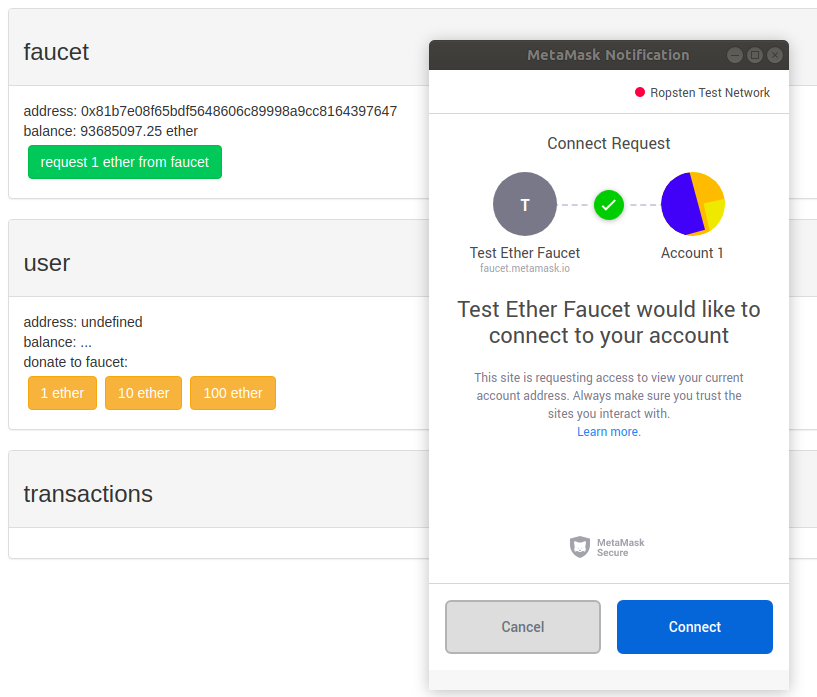
\includegraphics[scale=0.3,clip=false]{pictures/metamask-faucet.png}
  \end{center}

\end{frame}

\begin{frame}\frametitle{MetaMask: connect to the faucet}

  \begin{center}
    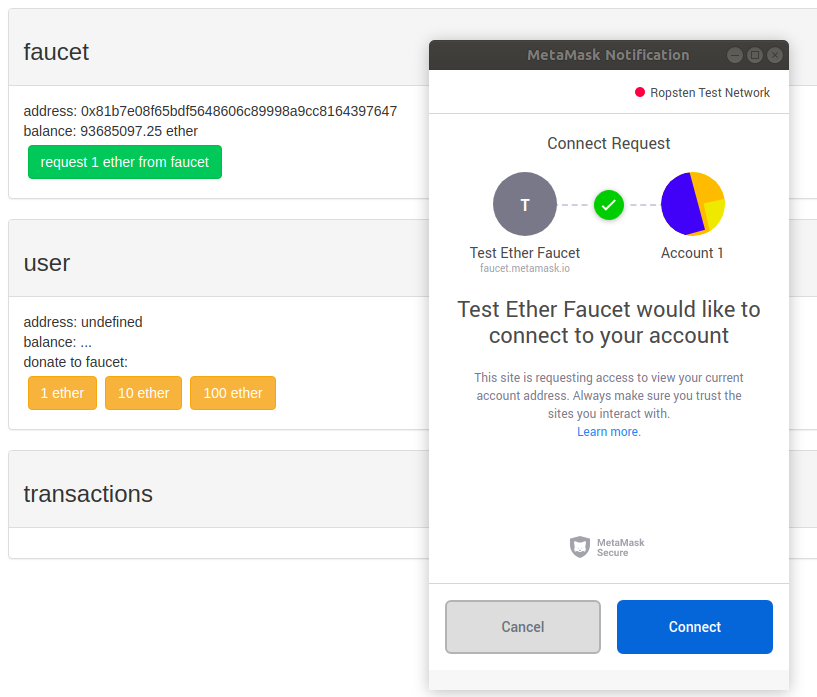
\includegraphics[scale=0.3,clip=false]{pictures/metamask-faucet.png}
  \end{center}

\end{frame}

\begin{frame}\frametitle{MetaMask: transaction for getting 1 ETH}

  \begin{center}
    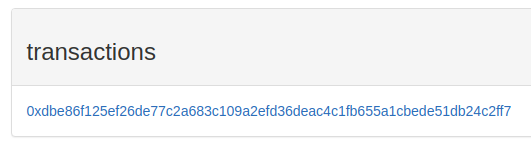
\includegraphics[width=\textwidth,clip=false]{pictures/metamask-faucet-transaction.png}
  \end{center}

\end{frame}

\begin{frame}\frametitle{MetaMask: detail of the transaction}

  \begin{center}
    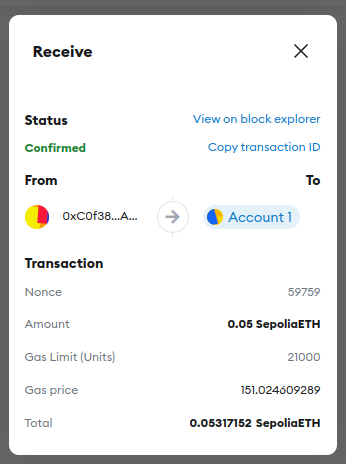
\includegraphics[scale=0.4,clip=false]{pictures/metamask-faucet-transaction-details.png}
  \end{center}

\end{frame}

\begin{frame}\frametitle{MetaMask: transactions of our account}

  \begin{center}
    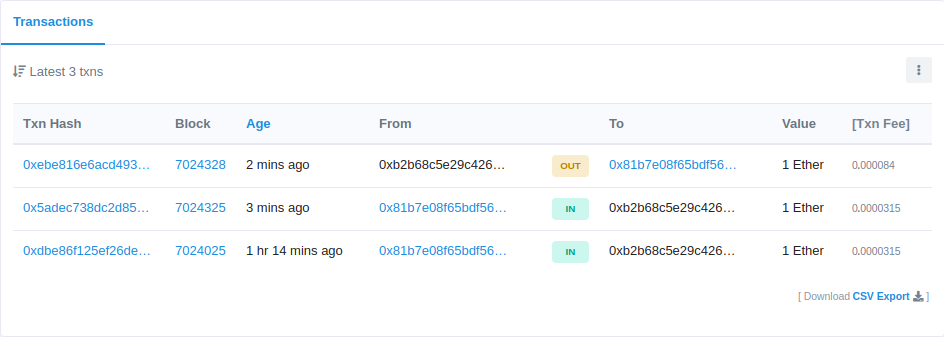
\includegraphics[width=\textwidth,clip=false]{pictures/metamask-faucet-transactions.png}
  \end{center}

\end{frame}

\begin{frame}\frametitle{Externally owned accounts (EOA) and contracts}

  \begin{greenbox}{}
    EOAs have keys, contracts have code. Both have an address
  \end{greenbox}
  
  \begin{center}
    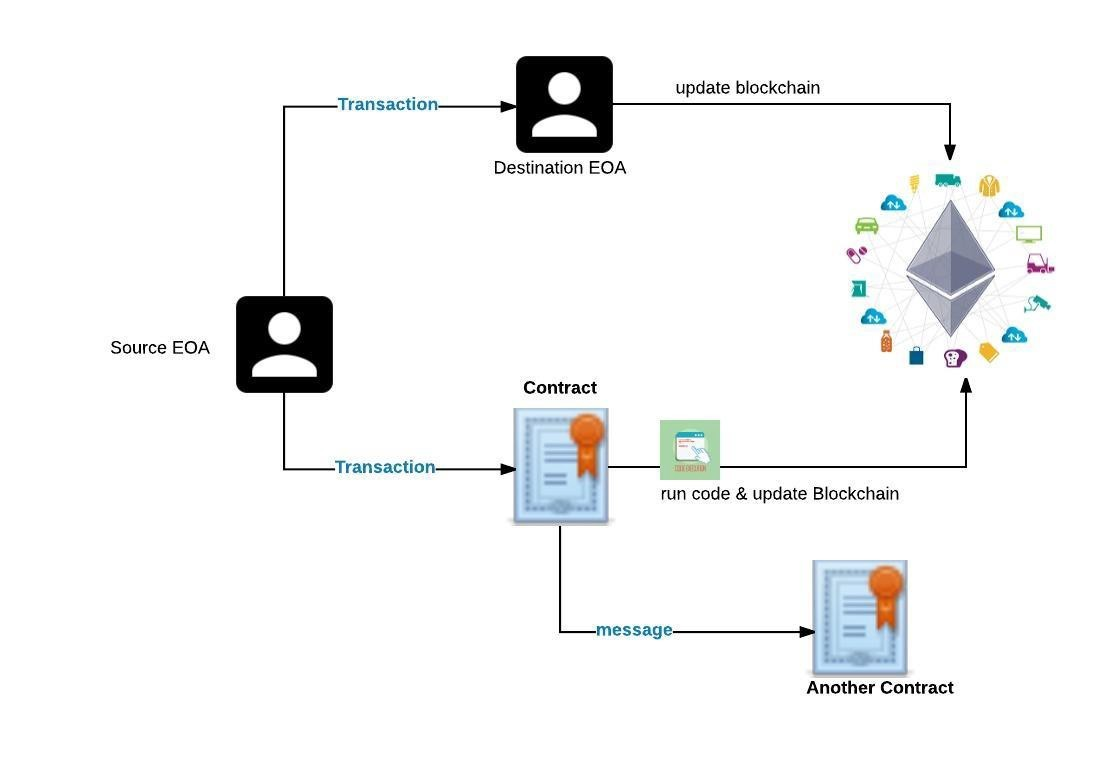
\includegraphics[scale=0.35,clip=false]{pictures/eoa-contract.jpg}
  \end{center}

\end{frame}

\begin{frame}\frametitle{Remix: web IDE for Solidity}

  \begin{greenbox}{}
    \url{https://remix.ethereum.org}
  \end{greenbox}

  \begin{center}
    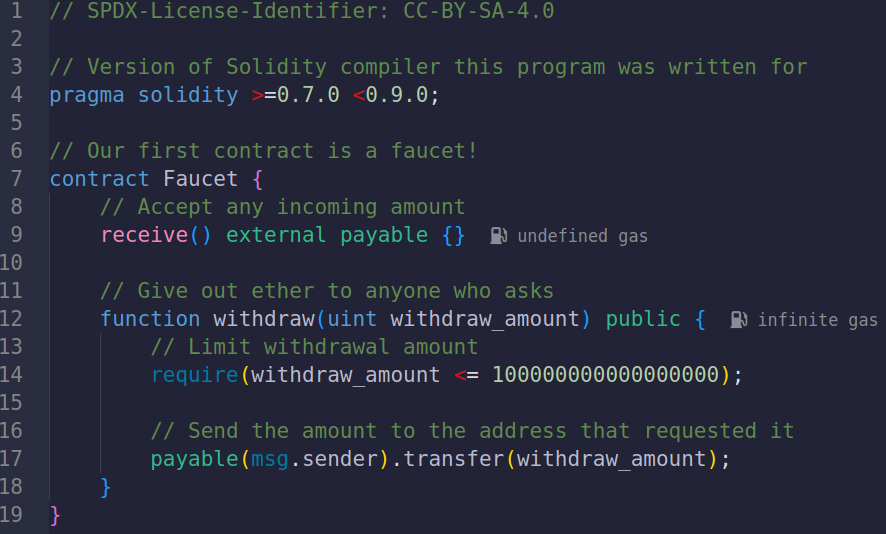
\includegraphics[width=\textwidth,clip=false]{pictures/faucet_sol.png}
  \end{center}

\end{frame}

\begin{frame}\frametitle{Remix: deploy an instance of the contract}

  \begin{greenbox}{}
    Remix will create for us a transaction with the 0 address as destination
  \end{greenbox}

  \begin{center}
    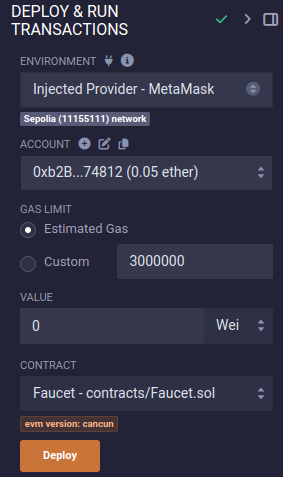
\includegraphics[scale=0.45,clip=false]{pictures/deploy-faucet.png}
  \end{center}

\end{frame}

\begin{frame}\frametitle{Remix: an instance of \<Faucet> has been deployed}

  \begin{center}
    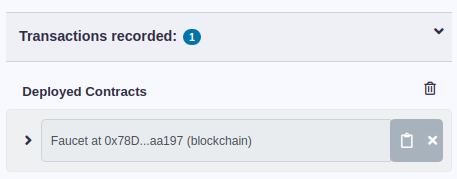
\includegraphics[width=\textwidth,clip=false]{pictures/deployed-faucet.png}
  \end{center}

\end{frame}

\begin{frame}\frametitle{Check the outcome on Etherscan}

  \begin{greenbox}{}
    \url{https://ropsten.etherscan.io}
  \end{greenbox}

  \begin{center}
    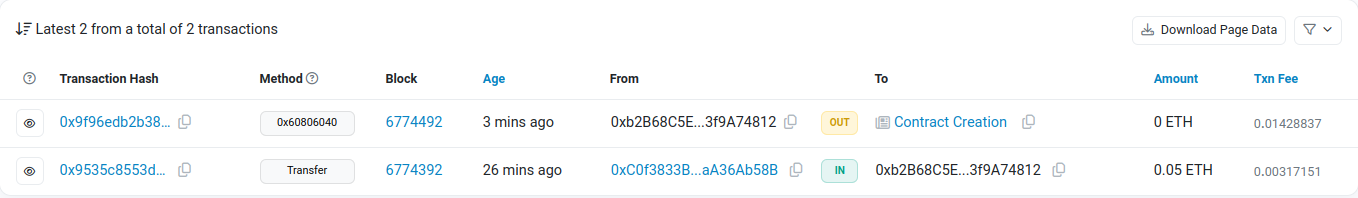
\includegraphics[width=\textwidth,clip=false]{pictures/faucet-etherscan.png}
  \end{center}

\end{frame}

\begin{frame}\frametitle{Send one Ether to the \<Faucet> through MetaMask}

  This corresponds to calling the default payable function
  
  \begin{center}
    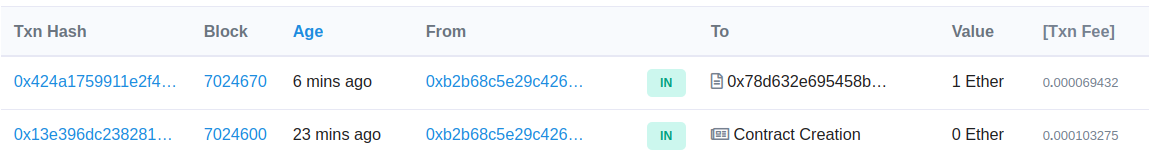
\includegraphics[width=\textwidth,clip=false]{pictures/faucet-etherscan2.png}
  \end{center}

\end{frame}

\begin{frame}\frametitle{Run the \<withdraw> function of the \<Faucet> in Remix}

  \begin{center}
    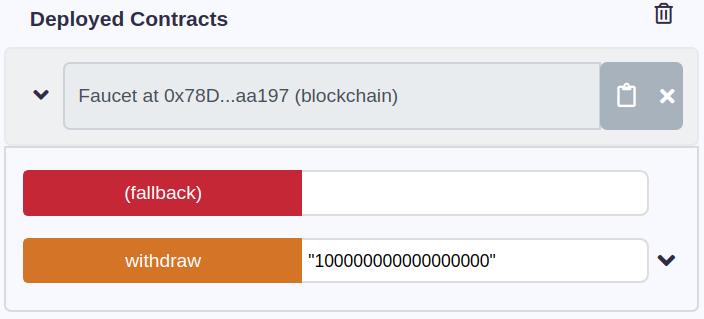
\includegraphics[width=\textwidth,clip=false]{pictures/faucet-withdraw.png}
  \end{center}

  \begin{center}
    $17$ zero's
  \end{center}
  
\end{frame}

\begin{frame}\frametitle{Check again on Etherscan}

  The faucet worked properly!
  
  \begin{center}
    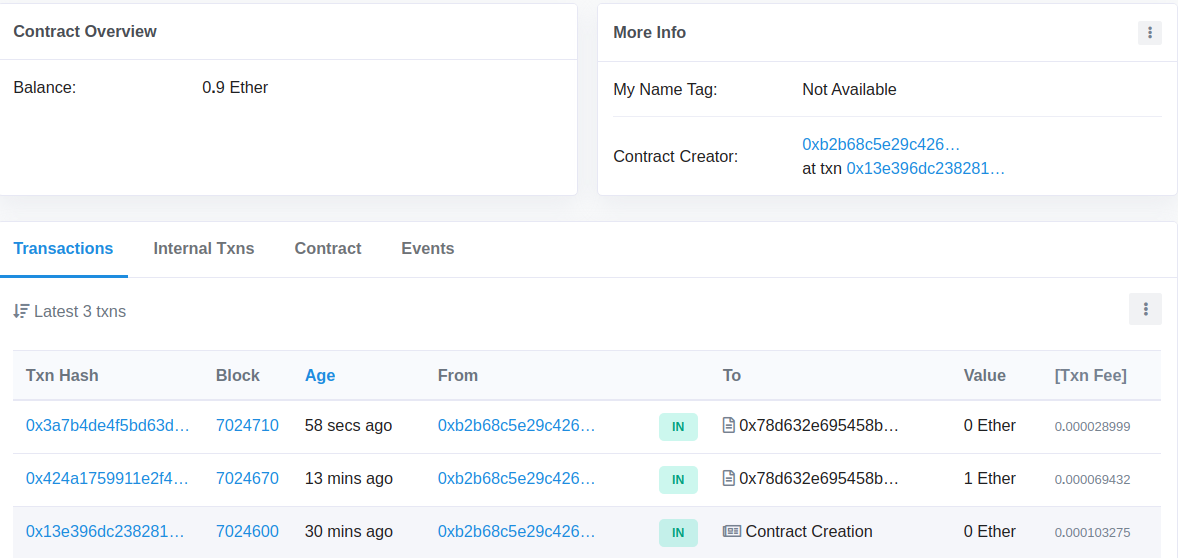
\includegraphics[width=\textwidth,clip=false]{pictures/faucet-etherscan3.png}
  \end{center}

\end{frame}

\begin{frame}\frametitle{The \<Faucet> has originated an internal transaction}

  \begin{center}
    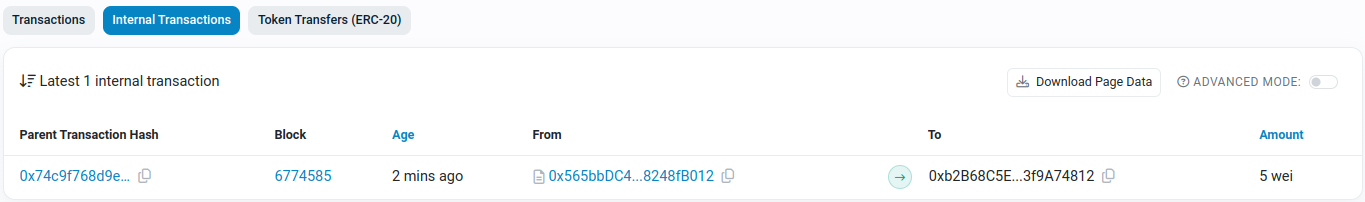
\includegraphics[width=\textwidth,clip=false]{pictures/faucet-etherscan-internal.png}
  \end{center}

  \begin{center}
    \<msg.sender.transfer(withdraw\_amount)>
  \end{center}

\end{frame}

\begin{frame}\frametitle{Ethereum clients}

  \begin{greenbox}{}
    An Ethereum client is a software application that implements
    the Ethereum specification (the \emph{Yellow Paper}) and communicates
    over the peer-to-peer network with other Ethereum clients.
  \end{greenbox}

  \medskip

  \begin{itemize}
  \item Parity (Rust)
  \item Geth (Go)
  \item \<cpp-ethereum> (C++)
  \item \<pyethereum> (Python)
  \item Mantis (Scala)
  \item Harmony (Java)
  \end{itemize}
  
\end{frame}

\begin{frame}\frametitle{Client types}

  \begin{greenbox}{Full nodes}
    A full node stores the whole blockchain ($\sim$200GB) and
    takes part in mining. Very slow to synchronize.
    It can query the blockchain offline and
    without letting a third party know the information that it's reading
  \end{greenbox}

  \bigskip

  \begin{greenbox}{Remote clients}
    A remote client does not store the blockchain but
    depends on another full node for operation. They are wallets
    that create and broadcast transactions (for instance, MetaMask)
  \end{greenbox}

  \bigskip

  \begin{greenbox}{Networks}
    The \emph{mainnet}, or a \emph{testnet}, or a local blockchain
    (Ganache)
  \end{greenbox}
  
\end{frame}

\begin{frame}\frametitle{Infura: a cloud service to a full node}

  \url{https://infura.io}

  \begin{center}
    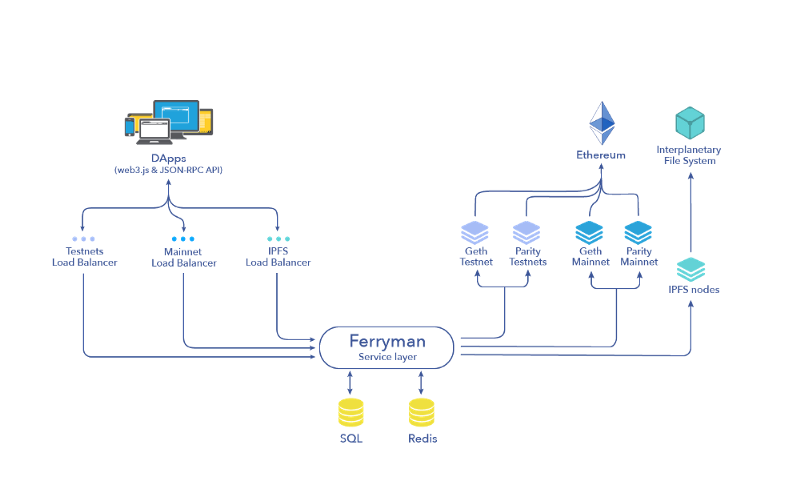
\includegraphics[width=\textwidth,clip=false]{pictures/infura.png}
  \end{center}

\end{frame}

\begin{frame}[fragile]\frametitle{Infura: ask for client version}

  \begin{greenbox}{}
    Register to Infura and create a project. Use the provided
    ID to build a query to Infura's JSON-RPC API:

\begin{semiverbatim}
$ \alert{curl https://mainnet.infura.io/v3/05....4
  -X POST
  -H "Content-Type: application/json"
  -d '\{"jsonrpc":"2.0","method":"web3_clientVersion",
  "params": [],"id":1\}'}
{\color{blue}\{"jsonrpc":"2.0","id":1,
 "result":"Geth/v1.9.9-omnibus-e320ae4c-20191206
               /linux-amd64/go1.13.4"\}}
\end{semiverbatim}

\end{greenbox}

\end{frame}

\begin{frame}[fragile]\frametitle{Infura: ask for gas price}

  \begin{greenbox}{}
    Use your Infura ID to build a query to Infura's JSON-RPC API:

\begin{semiverbatim}
$ \alert{curl https://mainnet.infura.io/v3/05....4
  -X POST
  -H "Content-Type: application/json"
  -d '\{"jsonrpc":"2.0","method":"eth_gasPrice",
       "params": [],"id":1\}'}
{\color{blue}\{"jsonrpc":"2.0","id":1,"result":"0x3b9aca00"\}}
$ \alert{echo $((0x3b9aca00))}
{\color{blue}1000000000}
\end{semiverbatim}

  \end{greenbox}

\end{frame}

\begin{frame}\frametitle{Infura implements Ethereum JSON-RPC API}

  \begin{center}
    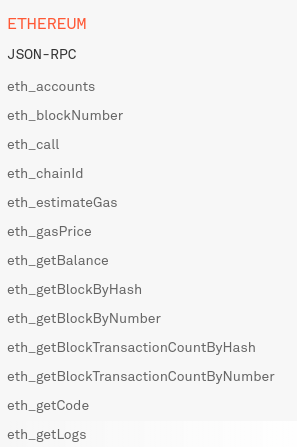
\includegraphics[scale=0.47,clip=false]{pictures/infura-json-rpc.png}
  \end{center}

\end{frame}

\begin{frame}[fragile]\frametitle{A Java client that connects to Infura}

  \begin{greenbox}{Use Eclipse to create a new Java Maven project}
    Add the following dependency to \<pom.xml>:
\begin{verbatim}
<project xmlns="http://maven.apache.org/POM/4.0.0"...>
  <modelVersion>4.0.0</modelVersion>
  <groupId>it.univr.ethereum</groupId>
  <artifactId>learning-ethereum</artifactId>
  <version>0.0.1-SNAPSHOT</version>
  <name>LearningEthereum</name>
  <dependencies>
    <dependency>
      <groupId>org.web3j</groupId>
      <artifactId>core</artifactId>
      <version>4.5.11</version>
    </dependency>
  </dependencies>
</project>
\end{verbatim}
  \end{greenbox}
\end{frame}

\begin{frame}[fragile]\frametitle{A Java client that connects to Infura}

{\small\begin{verbatim}
import java.io.IOException;

import org.web3j.protocol.Web3j;
import org.web3j.protocol.core.methods.response.Web3ClientVersion;
import org.web3j.protocol.http.HttpService;

public class ClientVersion {
  public static void main(String[] args) throws IOException {
    Web3j web3 = Web3j.build
      (new HttpService("https://ropsten.infura.io/v3/05...4"));
    Web3ClientVersion web3ClientVersion
      = web3.web3ClientVersion().send();
    System.out.println(web3ClientVersion.getWeb3ClientVersion());
  }
}
\end{verbatim}}

  \bigskip

  \url{https://javadoc.io/doc/org.web3j}

\end{frame}

\begin{frame}\frametitle{Mobile remote client: Jaxx}

  \begin{center}
    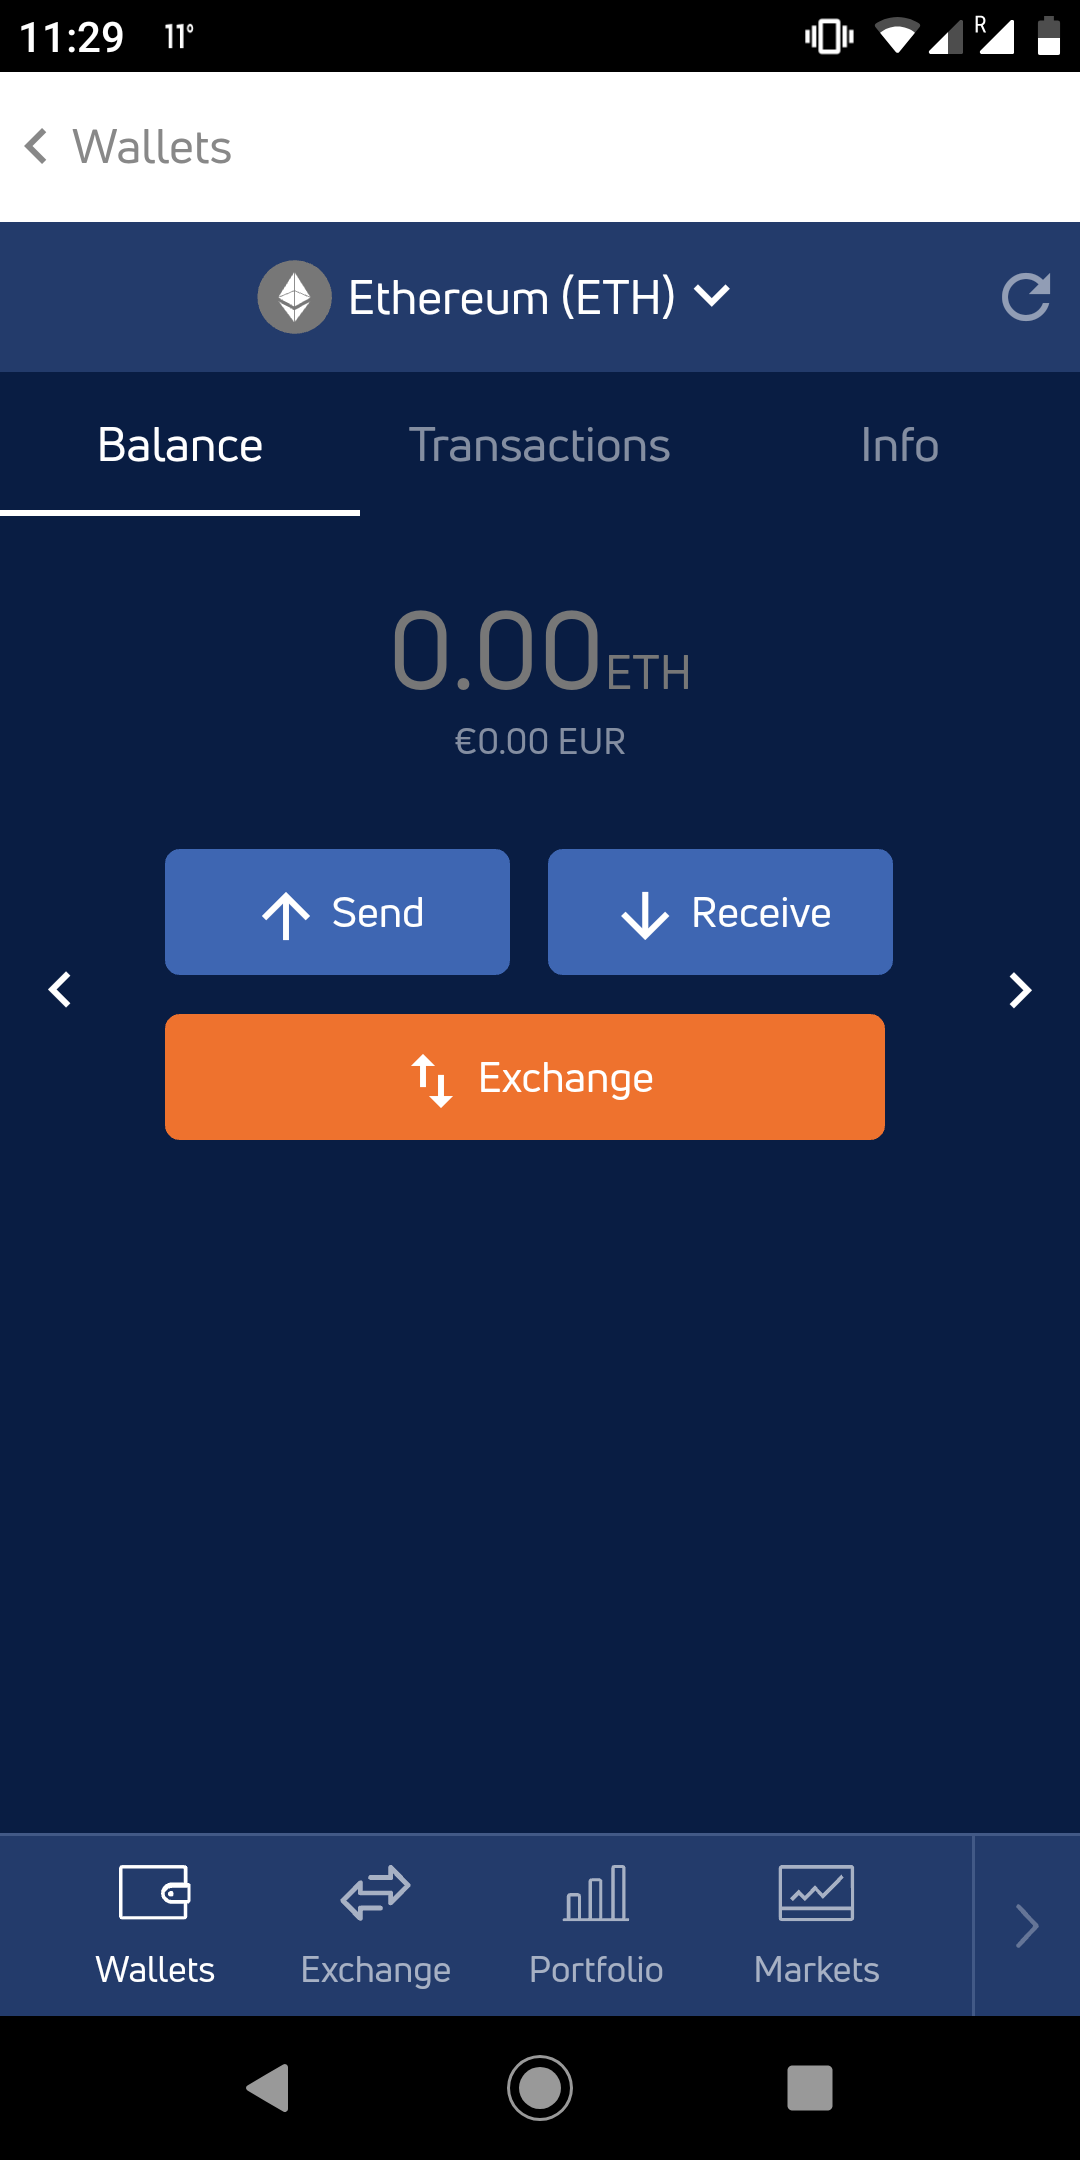
\includegraphics[scale=0.1,clip=false]{pictures/jaxx.png}
  \end{center}

\end{frame}

\end{document}
